\documentclass[
	ngerman,
	toc=listof, % Abbildungsverzeichnis sowie Tabellenverzeichnis in das Inhaltsverzeichnis aufnehmen
	toc=bibliography, % Literaturverzeichnis in das Inhaltsverzeichnis aufnehmen
	footnotes=multiple, % Trennen von direkt aufeinander folgenden Fußnoten
	parskip=half, % vertikalen Abstand zwischen Absätzen verwenden anstatt horizontale Einrückung von Folgeabsätzen
	numbers=noendperiod % Den letzten Punkt nach einer Nummerierung entfernen (nach DIN 5008)
]{scrartcl}
\pdfminorversion=5 % erlaubt das Einfügen von pdf-Dateien bis Version 1.7, ohne eine Fehlermeldung zu werfen (keine Garantie für fehlerfreies Einbetten!)
\usepackage[utf8]{inputenc} % muss als erstes eingebunden werden, da Meta/Packages ggfs. Sonderzeichen enthalten

% !TEX root = Projektdokumentation.tex

% Hinweis: der Titel muss zum Inhalt des Projekts passen und den zentralen Inhalt des Projekts deutlich herausstellen
\newcommand{\titel}{Schulze Methode}
\newcommand{\untertitel}{Algorithmus zum finden eines eindeutigen Siegers}
\newcommand{\kompletterTitel}{\titel{} -- \untertitel}

\newcommand{\autorName}{Steffen Holtkamp}
\newcommand{\autorMatrikelnummer}{201620684}
\newcommand{\autorAnschrift}{Thebenkamp 18}
\newcommand{\autorOrt}{46342 Velen}

\newcommand{\hochschulLogo}{whsLogo.png}
\newcommand{\betriebLogo}{LogoBetrieb.pdf}
\newcommand{\betriebName}{\textsc{Westfälische Hochschule - Bocholt}}
\newcommand{\betriebAnschrift}{ Münsterstraße 265}
\newcommand{\betriebOrt}{46397 Bocholt}

\newcommand{\ausbildungsberuf}{Informatik.Softwaresysteme}
\newcommand{\studiengang}{Informatik.Softwaresysteme}
\newcommand{\betreff}{Ausarbeitung spezielle Algorithmen}
\newcommand{\pruefungstermin}{Wintersemester 2018 - 2019}
\newcommand{\pruefer}{Prof. Dr. Martin Guddat}
\newcommand{\abgabeOrt}{Bocholt}
\newcommand{\abgabeTermin}{30.10.2018}
 % Metadaten zu diesem Dokument (Autor usw.)
% !TEX root = ../Projektdokumentation.tex

% Anpassung an Landessprache ---------------------------------------------------
\usepackage{babel}

% Umlaute ----------------------------------------------------------------------
%   Umlaute/Sonderzeichen wie äüöß direkt im Quelltext verwenden (CodePage).
%   Erlaubt automatische Trennung von Worten mit Umlauten.
% ------------------------------------------------------------------------------
\usepackage[T1]{fontenc}
\usepackage{textcomp} % Euro-Zeichen etc.

% Schrift ----------------------------------------------------------------------
\usepackage{lmodern} % bessere Fonts
\usepackage{relsize} % Schriftgröße relativ festlegen

% Tabellen ---------------------------------------------------------------------
\PassOptionsToPackage{table}{xcolor}
\usepackage{tabularx}
% für lange Tabellen
\usepackage{longtable}
\usepackage{array}
\usepackage{ragged2e}
\usepackage{lscape}
\newcolumntype{w}[1]{>{\raggedleft\hspace{0pt}}p{#1}} % Spaltendefinition rechtsbündig mit definierter Breite

% Grafiken ---------------------------------------------------------------------
\usepackage[dvips,final]{graphicx} % Einbinden von JPG-Grafiken ermöglichen
\usepackage{graphics} % keepaspectratio
\usepackage{floatflt} % zum Umfließen von Bildern
\graphicspath{{Bilder/}} % hier liegen die Bilder des Dokuments

% Sonstiges --------------------------------------------------------------------
\usepackage[titles]{tocloft} % Inhaltsverzeichnis DIN 5008 gerecht einrücken
\usepackage{amsmath,amsfonts} % Befehle aus AMSTeX für mathematische Symbole
\usepackage{enumitem} % anpassbare Enumerates/Itemizes
\usepackage{xspace} % sorgt dafür, dass Leerzeichen hinter parameterlosen Makros nicht als Makroendezeichen interpretiert werden

\usepackage{makeidx} % für Index-Ausgabe mit \printindex
\usepackage[printonlyused]{acronym} % es werden nur benutzte Definitionen aufgelistet

% Einfache Definition der Zeilenabstände und Seitenränder etc.
\usepackage{setspace}
\usepackage{geometry}

% Symbolverzeichnis
\usepackage[intoc]{nomencl}
\let\abbrev\nomenclature
\renewcommand{\nomname}{Abkürzungsverzeichnis}
\setlength{\nomlabelwidth}{.25\hsize}
\renewcommand{\nomlabel}[1]{#1 \dotfill}
\setlength{\nomitemsep}{-\parsep}

\usepackage{varioref} % Elegantere Verweise. „auf der nächsten Seite“
\usepackage{url} % URL verlinken, lange URLs umbrechen etc.

\usepackage{chngcntr} % fortlaufendes Durchnummerieren der Fußnoten
% \usepackage[perpage]{footmisc} % Alternative: Nummerierung der Fußnoten auf jeder Seite neu

\usepackage{ifthen} % bei der Definition eigener Befehle benötigt
\usepackage{todonotes} % definiert u.a. die Befehle \todo und \listoftodos
\usepackage[square]{natbib} % wichtig für korrekte Zitierweise

% PDF-Optionen -----------------------------------------------------------------
\usepackage{pdfpages}
\pdfminorversion=5 % erlaubt das Einfügen von pdf-Dateien bis Version 1.7, ohne eine Fehlermeldung zu werfen (keine Garantie für fehlerfreies Einbetten!)
\usepackage[
    bookmarks,
    bookmarksnumbered,
    bookmarksopen=true,
    bookmarksopenlevel=1,
    colorlinks=true,
% diese Farbdefinitionen zeichnen Links im PDF farblich aus
    linkcolor=AOBlau, % einfache interne Verknüpfungen
    anchorcolor=AOBlau,% Ankertext
    citecolor=AOBlau, % Verweise auf Literaturverzeichniseinträge im Text
    filecolor=AOBlau, % Verknüpfungen, die lokale Dateien öffnen
    menucolor=AOBlau, % Acrobat-Menüpunkte
    urlcolor=AOBlau,
% diese Farbdefinitionen sollten für den Druck verwendet werden (alles schwarz)
    %linkcolor=black, % einfache interne Verknüpfungen
    %anchorcolor=black, % Ankertext
    %citecolor=black, % Verweise auf Literaturverzeichniseinträge im Text
    %filecolor=black, % Verknüpfungen, die lokale Dateien öffnen
    %menucolor=black, % Acrobat-Menüpunkte
    %urlcolor=black,
%
    %backref, % Quellen werden zurück auf ihre Zitate verlinkt
    pdftex,
    plainpages=false, % zur korrekten Erstellung der Bookmarks
    pdfpagelabels=true, % zur korrekten Erstellung der Bookmarks
    hypertexnames=false, % zur korrekten Erstellung der Bookmarks
    linktocpage % Seitenzahlen anstatt Text im Inhaltsverzeichnis verlinken
]{hyperref}
% Befehle, die Umlaute ausgeben, führen zu Fehlern, wenn sie hyperref als Optionen übergeben werden
\hypersetup{
    pdftitle={\titel -- \untertitel},
    pdfauthor={\autorName},
    pdfcreator={\autorName},
    pdfsubject={\titel -- \untertitel},
    pdfkeywords={\titel -- \untertitel},
}


% zum Einbinden von Programmcode -----------------------------------------------
\usepackage{listings}
\usepackage{xcolor}
\definecolor{hellgelb}{rgb}{1,1,0.9}
\definecolor{colKeys}{rgb}{0,0,1}
\definecolor{colIdentifier}{rgb}{0,0,0}
\definecolor{colComments}{rgb}{0,0.5,0}
\definecolor{colString}{rgb}{1,0,0}
\lstset{
    float=hbp,
	basicstyle=\footnotesize,
    identifierstyle=\color{colIdentifier},
    keywordstyle=\color{colKeys},
    stringstyle=\color{colString},
    commentstyle=\color{colComments},
    backgroundcolor=\color{hellgelb},
    columns=flexible,
    tabsize=2,
    frame=single,
    extendedchars=true,
    showspaces=false,
    showstringspaces=false,
    numbers=left,
    numberstyle=\tiny,
    breaklines=true,
    breakautoindent=true,
	captionpos=b,
}
\lstdefinelanguage{cs}{
	sensitive=false,
	morecomment=[l]{//},
	morecomment=[s]{/*}{*/},
	morestring=[b]",
	morekeywords={
		abstract,event,new,struct,as,explicit,null,switch
		base,extern,object,this,bool,false,operator,throw,
		break,finally,out,true,byte,fixed,override,try,
		case,float,params,typeof,catch,for,private,uint,
		char,foreach,protected,ulong,checked,goto,public,unchecked,
		class,if,readonly,unsafe,const,implicit,ref,ushort,
		continue,in,return,using,decimal,int,sbyte,virtual,
		default,interface,sealed,volatile,delegate,internal,short,void,
		do,is,sizeof,while,double,lock,stackalloc,
		else,long,static,enum,namespace,string},
}
\lstdefinelanguage{natural}{
	sensitive=false,
	morecomment=[l]{/*},
	morestring=[b]",
	morestring=[b]',
	alsodigit={-,*},
	morekeywords={
		DEFINE,DATA,LOCAL,END-DEFINE,WRITE,CALLNAT,PARAMETER,USING,
		IF,NOT,END-IF,ON,*ERROR-NR,ERROR,END-ERROR,ESCAPE,ROUTINE,
		PERFORM,SUBROUTINE,END-SUBROUTINE,CONST,END-FOR,END,FOR,RESIZE,
		ARRAY,TO,BY,VALUE,RESET,COMPRESS,INTO,EQ},
}
\lstdefinelanguage{php}{
	sensitive=false,
	morecomment=[l]{/*},
	morestring=[b]",
	morestring=[b]',
	alsodigit={-,*},
	morekeywords={
		abstract,and,array,as,break,case,catch,cfunction,class,clone,const,
		continue,declare,default,do,else,elseif,enddeclare,endfor,endforeach,
		endif,endswitch,endwhile,extends,final,for,foreach,function,global,
		goto,if,implements,interface,instanceof,namespace,new,old_function,or,
		private,protected,public,static,switch,throw,try,use,var,while,xor
		die,echo,empty,exit,eval,include,include_once,isset,list,require,
		require_once,return,print,unset},
}
 % verwendete Packages
% !TEX root = ../Projektdokumentation.tex

% Seitenränder -----------------------------------------------------------------
\setlength{\topskip}{\ht\strutbox} % behebt Warnung von geometry
\geometry{a4paper,left=20mm,right=20mm,top=25mm,bottom=35mm}

\usepackage[
	automark, % Kapitelangaben in Kopfzeile automatisch erstellen
	headsepline, % Trennlinie unter Kopfzeile
	ilines % Trennlinie linksbündig ausrichten
]{scrpage2}

% Kopf- und Fußzeilen ----------------------------------------------------------
\pagestyle{scrheadings}
% chapterpagestyle gibt es nicht in scrartcl
%\renewcommand{\chapterpagestyle}{scrheadings}
\clearscrheadfoot

% Kopfzeile
\renewcommand{\headfont}{\normalfont} % Schriftform der Kopfzeile
\ihead{\large{\textsc{\titel}}\\ \small{\untertitel} \\[2ex] \textit{\headmark}}
\chead{}
\ohead{\includegraphics[scale=0.1]{\hochschulLogo}}
\setlength{\headheight}{15mm} % Höhe der Kopfzeile
%\setheadwidth[0pt]{textwithmarginpar} % Kopfzeile über den Text hinaus verbreitern (falls Logo den Text überdeckt)

% Fußzeile
\ifoot{\autorName}
\cfoot{}
\ofoot{\pagemark}

% Überschriften nach DIN 5008 in einer Fluchtlinie
% ------------------------------------------------------------------------------

% Abstand zwischen Nummerierung und Überschrift definieren
% > Schön wäre hier die dynamische Berechnung des Abstandes in Abhängigkeit
% > der Verschachtelungstiefe des Inhaltsverzeichnisses
\newcommand{\headingSpace}{1.5cm}

% Abschnittsüberschriften im selben Stil wie beim Inhaltsverzeichnis einrücken
\renewcommand*{\othersectionlevelsformat}[3]{
  \makebox[\headingSpace][l]{#3\autodot}
}

% Für die Einrückung wird das Paket tocloft benötigt
%\cftsetindents{chapter}{0.0cm}{\headingSpace}
\cftsetindents{section}{0.0cm}{\headingSpace}
\cftsetindents{subsection}{0.0cm}{\headingSpace}
\cftsetindents{subsubsection}{0.0cm}{\headingSpace}
\cftsetindents{figure}{0.0cm}{\headingSpace}
\cftsetindents{table}{0.0cm}{\headingSpace}


% Allgemeines
% ------------------------------------------------------------------------------

\onehalfspacing % Zeilenabstand 1,5 Zeilen
\frenchspacing % erzeugt ein wenig mehr Platz hinter einem Punkt

% Schusterjungen und Hurenkinder vermeiden
\clubpenalty = 10000
\widowpenalty = 10000
\displaywidowpenalty = 10000

% Quellcode-Ausgabe formatieren
\lstset{numbers=left, numberstyle=\tiny, numbersep=5pt, breaklines=true}
\lstset{emph={square}, emphstyle=\color{red}, emph={[2]root,base}, emphstyle={[2]\color{blue}}}

\counterwithout{footnote}{section} % Fußnoten fortlaufend durchnummerieren
\setcounter{tocdepth}{\subsubsectionlevel} % im Inhaltsverzeichnis werden die Kapitel bis zum Level der subsubsection übernommen
\setcounter{secnumdepth}{\subsubsectionlevel} % Kapitel bis zum Level der subsubsection werden nummeriert

% Aufzählungen anpassen
\renewcommand{\labelenumi}{\arabic{enumi}.}
\renewcommand{\labelenumii}{\arabic{enumi}.\arabic{enumii}.}
\renewcommand{\labelenumiii}{\arabic{enumi}.\arabic{enumii}.\arabic{enumiii}}

% Tabellenfärbung:
\definecolor{heading}{rgb}{0.64,0.78,0.86}
\definecolor{odd}{rgb}{0.9,0.9,0.9}
 % Definitionen zum Aussehen der Seiten
% !TEX root = ../Projektdokumentation.tex

% Abkürzungen, ggfs. mit korrektem Leerraum
\newcommand{\bs}{$\backslash$\xspace}
\newcommand{\bspw}{bspw.\xspace}
\newcommand{\bzw}{bzw.\xspace}
\newcommand{\ca}{ca.\xspace}
\newcommand{\dahe}{\mbox{d.\,h.}\xspace}
\newcommand{\etc}{etc.\xspace}
\newcommand{\eur}[1]{\mbox{#1\,\texteuro}\xspace}
\newcommand{\evtl}{evtl.\xspace}
\newcommand{\ggfs}{ggfs.\xspace}
\newcommand{\Ggfs}{Ggfs.\xspace}
\newcommand{\gqq}[1]{\glqq{}#1\grqq{}}
\newcommand{\inkl}{inkl.\xspace}
\newcommand{\insb}{insb.\xspace}
\newcommand{\ua}{\mbox{u.\,a.}\xspace}
\newcommand{\usw}{usw.\xspace}
\newcommand{\Vgl}{Vgl.\xspace}
\newcommand{\zB}{\mbox{z.\,B.}\xspace}
\newcommand{\condorcet}{Condorcet\xspace}
\newcommand{\condorcetParadox}{Condorcet-Paradoxon\xspace}
\newcommand{\condorcetSieger}{Condorcet-Sieger\xspace}
\newcommand{\schulze}{Schulze Methode\xspace}

% Befehle für häufig anfallende Aufgaben
\newcommand{\Abbildung}[1]{\autoref{fig:#1}}
\newcommand{\Anhang}[1]{\appendixname{}~\ref{#1}: \nameref{#1} \vpageref{#1}}
\newcommand{\includegraphicsKeepAspectRatio}[2]{\includegraphics[width=#2\textwidth,height=#2\textheight,keepaspectratio]{#1}}
\newcommand{\Zitat}[2][\empty]{\ifthenelse{\equal{#1}{\empty}}{\citep{#2}}{\citep[#1]{#2}}}
\newcommand{\Autor}[1]{\textsc{#1}} % zum Ausgeben von Autoren
\newcommand{\itemd}[2]{\item{\textbf{#1}}\\{#2}} % erzeugt ein Listenelement mit fetter Überschrift

% fügt Tabellen aus einer TEX-Datei ein
\newcommand{\tabelle}[3] % Parameter: caption, label, file
{\begin{table}[htbp]
\centering
\singlespacing
\input{Tabellen/#3}
\caption{#1}
\label{#2}
\end{table}}

\newcommand{\tabelleAnhang}[1] % Parameter: file
{\begin{center}
\singlespacing
\input{Tabellen/#1}
\end{center}}

% einfaches Wechseln der Schrift, z.B.: \changefont{cmss}{sbc}{n}
\newcommand{\changefont}[3]{\fontfamily{#1} \fontseries{#2} \fontshape{#3} \selectfont}

% Verwendung analog zu \includegraphics
\newlength{\myx} % Variable zum Speichern der Bildbreite
\newlength{\myy} % Variable zum Speichern der Bildhöhe
\newcommand\includegraphicstotab[2][\relax]{%
% Abspeichern der Bildabmessungen
\settowidth{\myx}{\includegraphics[{#1}]{#2}}%
\settoheight{\myy}{\includegraphics[{#1}]{#2}}%
% das eigentliche Einfügen
\parbox[c][1.1\myy][c]{\myx}{%
\includegraphics[{#1}]{#2}}%
}

\definecolor{AOBlau}{rgb}{0, 0.28, 0.56}

% verschiedene Befehle um Wörter semantisch auszuzeichnen ----------------------
\newcommand{\Index}[2][\empty]{\ifthenelse{\equal{#1}{\empty}}{\index{#2}#2}{\index{#1}#2}}
\newcommand{\Fachbegriff}[2][\empty]{\ifthenelse{\equal{#1}{\empty}}{\textit{\Index{#2}}}{\textit{\Index[#1]{#2}}}}
\newcommand{\NeuerBegriff}[2][\empty]{\ifthenelse{\equal{#1}{\empty}}{\textbf{\Index{#2}}}{\textbf{\Index[#1]{#2}}}}

\newcommand{\Ausgabe}[1]{\texttt{#1}}
\newcommand{\Eingabe}[1]{\texttt{#1}}
\newcommand{\Code}[1]{\texttt{#1}}
\newcommand{\Datei}[1]{\texttt{#1}}

\newcommand{\Assembly}[1]{\textsf{#1}}
\newcommand{\Klasse}[1]{\textsf{#1}}
\newcommand{\Methode}[1]{\textsf{#1}}
\newcommand{\Attribut}[1]{\textsf{#1}}

\newcommand{\Datentyp}[1]{\textsf{#1}}
\newcommand{\XMLElement}[1]{\textsf{#1}}
\newcommand{\Webservice}[1]{\textsf{#1}}

\newcommand{\Refactoring}[1]{\Fachbegriff{#1}}
\newcommand{\CodeSmell}[1]{\Fachbegriff{#1}}
\newcommand{\Metrik}[1]{\Fachbegriff{#1}}
\newcommand{\DesignPattern}[1]{\Fachbegriff{#1}}


 % eigene allgemeine Befehle, die z.B. die Arbeit mit LaTeX erleichtern
% !TEX root = ../Projektdokumentation.tex

% Abkürzungen, ggfs. mit korrektem Leerraum
\newcommand{\bs}{$\backslash$\xspace}
\newcommand{\bspw}{bspw.\xspace}
\newcommand{\bzw}{bzw.\xspace}
\newcommand{\ca}{ca.\xspace}
\newcommand{\dahe}{\mbox{d.\,h.}\xspace}
\newcommand{\etc}{etc.\xspace}
\newcommand{\eur}[1]{\mbox{#1\,\texteuro}\xspace}
\newcommand{\evtl}{evtl.\xspace}
\newcommand{\ggfs}{ggfs.\xspace}
\newcommand{\Ggfs}{Ggfs.\xspace}
\newcommand{\gqq}[1]{\glqq{}#1\grqq{}}
\newcommand{\inkl}{inkl.\xspace}
\newcommand{\insb}{insb.\xspace}
\newcommand{\ua}{\mbox{u.\,a.}\xspace}
\newcommand{\usw}{usw.\xspace}
\newcommand{\Vgl}{Vgl.\xspace}
\newcommand{\zB}{\mbox{z.\,B.}\xspace}
\newcommand{\condorcet}{Condorcet\xspace}
\newcommand{\condorcetParadox}{Condorcet-Paradoxon\xspace}
\newcommand{\condorcetSieger}{Condorcet-Sieger\xspace}
\newcommand{\schulze}{Schulze Methode\xspace}

% Befehle für häufig anfallende Aufgaben
\newcommand{\Abbildung}[1]{\autoref{fig:#1}}
\newcommand{\Anhang}[1]{\appendixname{}~\ref{#1}: \nameref{#1} \vpageref{#1}}
\newcommand{\includegraphicsKeepAspectRatio}[2]{\includegraphics[width=#2\textwidth,height=#2\textheight,keepaspectratio]{#1}}
\newcommand{\Zitat}[2][\empty]{\ifthenelse{\equal{#1}{\empty}}{\citep{#2}}{\citep[#1]{#2}}}
\newcommand{\Autor}[1]{\textsc{#1}} % zum Ausgeben von Autoren
\newcommand{\itemd}[2]{\item{\textbf{#1}}\\{#2}} % erzeugt ein Listenelement mit fetter Überschrift

% fügt Tabellen aus einer TEX-Datei ein
\newcommand{\tabelle}[3] % Parameter: caption, label, file
{\begin{table}[htbp]
\centering
\singlespacing
\input{Tabellen/#3}
\caption{#1}
\label{#2}
\end{table}}

\newcommand{\tabelleAnhang}[1] % Parameter: file
{\begin{center}
\singlespacing
\input{Tabellen/#1}
\end{center}}

% einfaches Wechseln der Schrift, z.B.: \changefont{cmss}{sbc}{n}
\newcommand{\changefont}[3]{\fontfamily{#1} \fontseries{#2} \fontshape{#3} \selectfont}

% Verwendung analog zu \includegraphics
\newlength{\myx} % Variable zum Speichern der Bildbreite
\newlength{\myy} % Variable zum Speichern der Bildhöhe
\newcommand\includegraphicstotab[2][\relax]{%
% Abspeichern der Bildabmessungen
\settowidth{\myx}{\includegraphics[{#1}]{#2}}%
\settoheight{\myy}{\includegraphics[{#1}]{#2}}%
% das eigentliche Einfügen
\parbox[c][1.1\myy][c]{\myx}{%
\includegraphics[{#1}]{#2}}%
}

\definecolor{AOBlau}{rgb}{0, 0.28, 0.56}

% verschiedene Befehle um Wörter semantisch auszuzeichnen ----------------------
\newcommand{\Index}[2][\empty]{\ifthenelse{\equal{#1}{\empty}}{\index{#2}#2}{\index{#1}#2}}
\newcommand{\Fachbegriff}[2][\empty]{\ifthenelse{\equal{#1}{\empty}}{\textit{\Index{#2}}}{\textit{\Index[#1]{#2}}}}
\newcommand{\NeuerBegriff}[2][\empty]{\ifthenelse{\equal{#1}{\empty}}{\textbf{\Index{#2}}}{\textbf{\Index[#1]{#2}}}}

\newcommand{\Ausgabe}[1]{\texttt{#1}}
\newcommand{\Eingabe}[1]{\texttt{#1}}
\newcommand{\Code}[1]{\texttt{#1}}
\newcommand{\Datei}[1]{\texttt{#1}}

\newcommand{\Assembly}[1]{\textsf{#1}}
\newcommand{\Klasse}[1]{\textsf{#1}}
\newcommand{\Methode}[1]{\textsf{#1}}
\newcommand{\Attribut}[1]{\textsf{#1}}

\newcommand{\Datentyp}[1]{\textsf{#1}}
\newcommand{\XMLElement}[1]{\textsf{#1}}
\newcommand{\Webservice}[1]{\textsf{#1}}

\newcommand{\Refactoring}[1]{\Fachbegriff{#1}}
\newcommand{\CodeSmell}[1]{\Fachbegriff{#1}}
\newcommand{\Metrik}[1]{\Fachbegriff{#1}}
\newcommand{\DesignPattern}[1]{\Fachbegriff{#1}}


 % eigene projektspezifische Befehle, z.B. Abkürzungen usw.

\begin{document}
\linenumbers
\phantomsection
\thispagestyle{plain}
\pdfbookmark[1]{Deckblatt}{deckblatt}
% !TEX root = Projektdokumentation.tex
\begin{titlepage}

\begin{center}

\Large{\studiengang}\\
\LARGE{\betreff}\\[4ex]

\huge{\textbf{\titel}}\\[1.5ex]
\Large{\textbf{\untertitel}}\\[4ex]

\normalsize
Abgabetermin: \abgabeOrt, den \abgabeTermin \\
Wintersemester: 2018/2019 
\\[3em]

\textbf{Student:}\\
\autorName\\
Matrikelnummer: \autorMatrikelnummer\\[5ex]


\includegraphics[scale=0.4]{\hochschulLogo}\\[2ex]
\betriebName\\
\pruefer\\
\betriebAnschrift\\
\betriebOrt\\[5em]

\end{center}


\end{titlepage}
\cleardoublepage

% Preface --------------------------------------------------------------------
\phantomsection
\pagenumbering{Roman}
\pdfbookmark[1]{Inhaltsverzeichnis}{inhalt}
\tableofcontents
\cleardoublepage

\phantomsection
\listoffigures
\cleardoublepage

\phantomsection
\listoftables
\cleardoublepage

\phantomsection
\lstlistoflistings
\cleardoublepage

\newcommand{\abkvz}{Abkürzungsverzeichnis}
\renewcommand{\nomname}{\abkvz}
\section*{\abkvz}
\markboth{\abkvz}{\abkvz}
\addcontentsline{toc}{section}{\abkvz}
% !TEX root = Projektdokumentation.tex

% Es werden nur die Abkürzungen aufgelistet, die mit \ac definiert und auch benutzt wurden. 
%
% \acro{VERSIS}{Versicherungsinformationssystem\acroextra{ (Bestandsführungssystem)}}
% Ergibt in der Liste: VERSIS Versicherungsinformationssystem (Bestandsführungssystem)
% Im Text aber: \ac{VERSIS} -> Versicherungsinformationssystem (VERSIS)

% Hinweis: allgemein bekannte Abkürzungen wie z.B. bzw. u.a. müssen nicht ins Abkürzungsverzeichnis aufgenommen werden
% Hinweis: allgemein bekannte IT-Begriffe wie Datenbank oder Programmiersprache müssen nicht erläutert werden,
%          aber ggfs. Fachbegriffe aus der Domäne des Prüflings (z.B. Versicherung)

% Die Option (in den eckigen Klammern) enthält das längste Label oder
% einen Platzhalter der die Breite der linken Spalte bestimmt.
\begin{acronym}[WWWWW]
	\acro{AO}{\textsc{Alte Oldenburger} Krankenversicherung AG}
	\acro{API}{Application Programming Interface}
	\acro{CSS}{Cascading Style Sheets}
	\acro{CSV}{Comma Separated Value}
	\acro{EPK}{Ereignisgesteuerte Prozesskette}
	\acro{ERM}{En\-ti\-ty-Re\-la\-tion\-ship-Mo\-dell}
	\acro{HTML}{Hypertext Markup Language}\acused{HTML}
	\acro{IDE}{Integrated Development Environment}
	\acro{MVC}[MVC]{Model View Controller}
	\acro{NatInfo}[\textsc{NatInfo}]{Natural Information System}
	\acro{Natural}[\textsc{Natural}]{Programmiersprache der Software AG}\acused{Natural}
	\acro{ORM}{Object-Relational Mapping}
	\acro{PHP}{Hypertext Preprocessor}
	\acro{SDK}{Software Development Kit}
	\acro{SQL}{Structured Query Language}
	\acro{SVN}{Subversion}
	\acro{UML}{Unified Modeling Language}
	\acro{XML}{Extensible Markup Language}
\end{acronym}

\clearpage

% Inhalt ---------------------------------------------------------------------
\pagenumbering{arabic}
% !TEX root = Projektdokumentation.tex
% !TEX root = ../Projektdokumentation.tex
\section{Einleitung}
\label{sec:Einleitung}


\subsection{Markus Schulze} 
\label{sec:markusSchulze}
Wer war Markus Schulze


\subsection{Problemstellung} 
\label{sec:problemstellung}
Welches Problem soll diese Methode lösen?

\subsection{Anforderungen} 
\label{sec:anforderungen}
Welche Anforderungen werden an einen solchen Algorithmus gestellt.






% !TEX root = ../Projektdokumentation.tex
\section{Definition}
\label{sec:definition}


\subsection{Voraussetzungen} 
\label{sec:voraussetzungen}
Es gibt einige Voraussetzungen, die eine Wahl erfüllen muss, damit man die Schulze Methode auf diese Wahl anwenden kann.

\begin{enumerate}
\item Es werden Kandidaten benötigt, die sich zur Wahl stellen. Hierbei muss es mindestens zwei Kandidaten geben, da sonst keine Rangfolge erstellt werden kann. Bei zwei Kandidaten ist die Lösung jedoch trivial, da dort der Gewinner der Kandidat ist, der am häufigsten, von den Wählern dem Gegner vorgezogen wurde.

Mathematische Definition:
Sei A eine endliche nicht leere Menge an Kandidaten. Wobei die Anzahl der Kandidaten C ist und gilt: 
\[
  C \in\ \mathbb{N}\  und \ 1 < C <\ \infty
\]

\item Jeder Wähler ordnet die Kandidaten eine Zahl zu und aus dieser Zahl wird eine Rangfolge erstellt. Je kleiner die Zahl ist desto höher ist die Platzierung. Hierbei ist die Größe der Zahl oder der Abstand uninteressant, da nur die Rangfolge betrachtet wird.

Des weiteren gilt:
\begin{enumerate}
\item \label{itm:Regel1} Es können mehrere Kandidaten den gleichen Rang haben, dass bedeutet, dass kein Kandidat dem anderen Kandidaten auf der selben Platzierung vorgezogen wird. 
\item Wenn ein Wähler keine Bewertung für einen Kandidaten abgibt, werden alle Kandidaten, die eine Bewertung haben, diesem Kandidaten vorgezogen. Werden mehrere Kandidaten nicht bewertet, werden sie wir im vorherigen Punkt bewertet.
\end{enumerate}



\end{enumerate}


\subsection{Theoretische Grundlagen} 
\label{sec:theoretische Grundlagen}
Welche mathematische Berechnung wird zur Lösung dieses Problems eingesetzt? Welche Theorie wurde entwickelt




% !TEX root = ../Projektdokumentation.tex
\section{Beispiel 1}
\label{sec:beispiel1}


\subsection{Ausgangssituation} 
\label{sec:ausgangssituation1}
Welche Daten sind Vorhanden 


\subsection{Lösungsschritte} 
\label{sec:loesungen1}
Bilder Tabellen um zur Lösung zu gelangen. Auch Mathematisch

\subsection{Ergebnis} 
\label{sec:ergebnis1}
Welches Erkenntnis haben wir gezogen.



% !TEX root = Projektdokumentation.tex
\section{Beispiel 2}
\label{sec:beispiel2}

\subsection{Ausgangssituation} 
\label{sec:ausgangssituation2}
Als Ausgangsmethode kann, wie in Beispiel 1 (Abschnitt: \ref{sec:ausgangssituation1}) wieder eine Wahl eines Kurssprechers angenommen werden. 

In dieser Wahl haben 21 Personen die Kandidaten $a$ bis $d$ in eine Reihenfolge sortiert, dabei hat sich diese Verteilung eingestellt

\begin{description}
\centering
\item[8 mal] $a \succ_{v} c \succ_{v} d \succ_{v}b$
\item[2 mal] $b \succ_{v} a \succ_{v} d \succ_{v}c$
\item[4 mal] $c \succ_{v} d \succ_{v} b \succ_{v}a$
\item[4 mal] $d \succ_{v} b \succ_{v} a \succ_{v}c$
\item[3 mal] $d \succ_{v} c \succ_{v} b \succ_{v}a$
\end{description}



\subsection{Lösungsschritte} 
\label{sec:loesungen2}
Zuerst werden die Kandidaten wieder gegeneinander aufgestellt.

 \begin{description}
 \centering
 \item[$a$ vs. $b$] 8 Stimmen gegen 13 Stimmen, $b$ gewinnt
 \item[$a$ vs. $c$] 14 Stimmen gegen 7 Stimmen, $a$ gewinnt
 \item[$a$ vs. $d$] 10 Stimmen gegen 11 Stimmen, $d$ gewinnt
 \item[$b$ vs. $c$] 6 Stimmen gegen 15 Stimmen, $c$ gewinnt
 \item[$b$ vs. $d$] 2 Stimmen gegen 19 Stimmen, $d$ gewinnt
 \item[$c$ vs. $d$] 12 Stimmen gegen 9 Stimmen, $c$ gewinnt
 \end{description}
 
In diesem Fall sieht man, dass es keinen \condorcetSieger gibt, also das es kein Kandidaten gibt, der es geschafft hat alle Gegner im Zweikampf zu überholen, diese Situation ist das sogenannte \condorcetParadox. \citep{EnricoSchoebel2018}

\newpage
Die \schulze kann diese Problem jedoch lösen indem, wie in Tabelle \ref{beispiel2N} dargestellt, die Menge $N$ gebildet wird.

% !TEX root = Projektdokumentation.tex

\begin{longtable}[c]{|l|l|l|l|l|}
\hline
            & N{[}*,a{]} & N{[}*,b{]} & N{[}*,c{]} & N{[}*,d{]} \\ \hline
\endfirsthead
%
\endhead
%
N{[}a, *{]} & ---        & 8          & 14         & 10         \\ \hline
N{[}b, *{]} & 13         & ---        & 6          & 2          \\ \hline
N{[}c, *{]} & 7          & 15         & ---        & 12         \\ \hline
N{[}d, *{]} & 11         & 19         & 9          & ---        \\ \hline
\caption{Die Menge $N$ (Beispiel 2)}
\label{beispiel2N}\\
\end{longtable}

Aus der Menge $N$ wird der Graph gebildet, siehe Abbildung \ref{fig:graph2}.

\begin{figure}[!h]
\centering
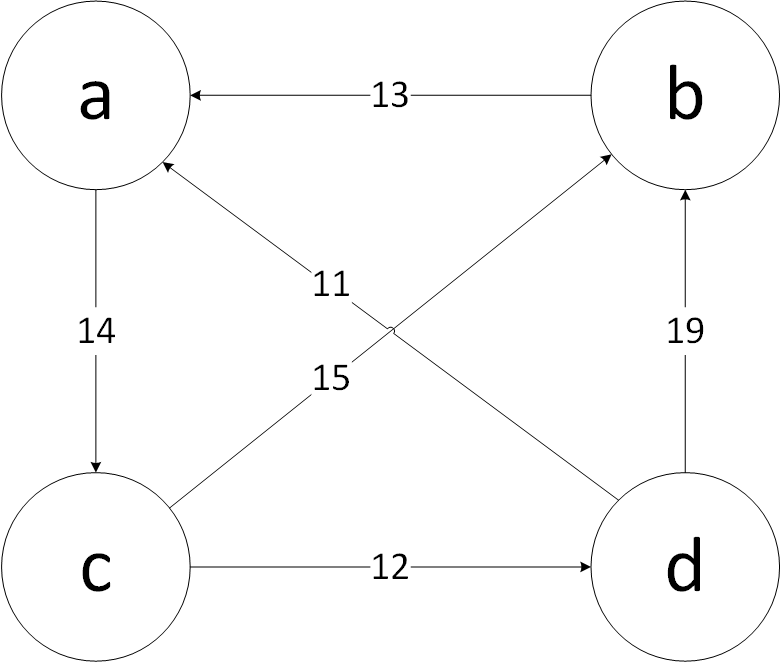
\includegraphics[scale=0.5]{Bilder/Beispiel2_Graph.png}
\caption{Graph über die Menge $N$(Beispiel 2)}
\label{fig:graph2}
\end{figure}

Nun werden wieder die stärksten Pfade gesucht und in die Menge $P$ eingefügt, die in Tabelle \ref{beispiel2p} zu sehen ist.

% !TEX root = ../Projektdokumentation.tex

\begin{longtable}[c]{|l|l|l|l|l|}
\hline
             & P{[}*,a{]} & P{[}*,b{]} & P{[}*,c{]} & P{[}*,d{]} \\ \hline
\endfirsthead
%
\endhead
%
PN{[}a, *{]} & ---        & 14         & 14         & 12         \\ \hline
PN{[}b, *{]} & 13         & ---        & 13         & 12         \\ \hline
P{[}c, *{]}  & 13         & 15         & ---        & 12         \\ \hline
P{[}d, *{]}  & 13         & 19         & 13         & ---        \\ \hline
\caption{Die Menge $P$ in Beispiel 2}
\label{beispiel2p}\\
\end{longtable}

Anschließend wird mit den Werten der Menge $P$ die neu Zweikampfsituation erstellt und man erhält die Relation $\mathcal{O} = \{ ab,ac,cb,da,db,dc \}$


\subsection{Ergebnis} 
\label{sec:ergebnis2}
Analog zu Beispiel 1 (Abschnitt \ref{sec:beispiel1}) wird die Relation $\mathcal{O}$ untersucht, um die Menge der Sieger zu finden. In diesem Fall ist $\mathcal{S}=\{d\}$  und der Sieger ist Kandidat $d$. Hier sieht man, dass die \schulze Probleme anderer Wahlverfahren lösen kann.

Eine Ausführliche Besprechung, wie in Beispiel 1 kann in der orginal Ausarbeitung von Martin Schulze in Kapitel 3.1 nachgelesen werden. \citep{Schulze2017}

% !TEX root = Projektdokumentation.tex
\section{Beispiel 3}
\label{sec:beispiel3}

\subsection{Ausgangssituation} 
\label{sec:ausgangssituation3}
In Abschnitt \ref{sec:voraussetzungen} wurde beschrieben, dass die Schulze Methode auch Ergebnisse liefert, wenn Kandidaten gleich oder nicht bewertet wurden. Nicht bewertete Kandidaten werden dabei behandelt, als wären sie alle vom Wähler auf dem letzten Platz gewählt worden, sodass jeder Kandidat, der vom Wähler bewertet wurde, den nicht bewerteten Kandidaten vorgezogen wird. Diese Beispiel Bezieht sich auf das sechste Beispiel von Martin Schulze in Kapitel 3.6 \citep{Schulze2017}.

\begin{description}
\centering
\item[6 mal] $a \succ_{v} b \succ_{v} c \succ_{v}d$
\item[8 mal] $a \approx_{v} b \succ_{v} c \approx_{v}d$
\item[8 mal] $a \approx_{v} c \succ_{v} b \approx_{v}d$
\item[18 mal] $a \approx_{v} c \succ_{v} d \succ_{v}b$
\item[8 mal] $a \approx_{v} c \approx_{v} d \succ_{v}d$
\item[40 mal] $b \succ_{v} a \approx_{v} c \approx_{v}d$
\item[4 mal] $c \succ_{v} b \succ_{v} d \succ_{v}a$
\item[9 mal] $c \succ_{v} d \succ_{v} a \succ_{v}b$
\item[8 mal] $c \approx_{v} d \succ_{v} a \approx_{v}b$
\item[14 mal] $d \succ_{v} a \succ_{v} b \succ_{v}c$
\item[11 mal] $d \succ_{v} b \succ_{v} c \succ_{v}a$
\item[4 mal] $d \succ_{v} c \succ_{v} a \succ_{v}b$
\end{description}

Zur Erläuterung wird die Wahl $a \approx_{v} b \succ_{v} c \approx_{v}d$ betrachtet. Hier hat der Wähler gesagt, er möchte lieber Kandidat $a$ oder $b$ haben, welcher ist ihm dabei egal, aber lieber einen von den beiden Kandidaten, als die Kandidaten $b$ oder $d$. Dort macht der Wähler aber auch kein Unterschied ob $b$ oder $d$ beide findet er gleich gut/schlecht.

\subsection{Lösungsschritte} 
\label{sec:loesungen3}
Als erstes muss die Menge $N$ bestimmen werden, in der man die Kandidaten gegeneinander antreten lässt, nur kann es diesmal zu Duellen ohne Sieger kommen, da beide Kandidaten gleich bewertet wurden. Diese Stimmen werden dann nicht Berücksichtigt. 

Exemplarisch wird in Tabelle \ref{beispiel3ab} das Duell von Kandidat $a$ gegen Kandidat $b$ dargestellt. 

% !TEX root = Projektdokumentation.tex

\begin{longtable}[c]{|l|l|l|l|}
\hline
Duelle & $a$  & $b$  & Sieger \\ \hline
\endfirsthead
%
\endhead
%
1      & 6  &    & $a$      \\ \hline
\rowcolor[HTML]{9B9B9B} 
2      & 8  & 8  & keiner \\ \hline
3      & 8  &    & $a$      \\ \hline
4      & 18 &    & $a$     \\ \hline
5      & 8  &    & $a$    \\ \hline
6      &    & 40 & $b$    \\ \hline
7      &    & 4  & $b$     \\ \hline
8      & 9  &    & $a$    \\ \hline
\rowcolor[HTML]{9B9B9B} 
9      & 8  & 8  & keiner \\ \hline
10     & 14 &    & $a$    \\ \hline
11     &    & 11 & $b$    \\ \hline
12     & 4  &    & $a$    \\ \hline
Summe  & 67 & 55 &        \\ \hline
\caption{Duell $a$ gegen $b$, graue Felder sind nicht bewertet, da unentschieden (Beispiel 3)}
\label{beispiel3ab}\\
\end{longtable}


Wenn man dieses Verfahren für alle Kandidaten anwendet erhält man die Menge $N$, die in Tabelle \ref{beispiel3N} aufgetragen ist.

% !TEX root = Projektdokumentation.tex

\begin{longtable}[c]{|l|l|l|l|l|}
\hline
            & N{[}*,a{]} & N{[}*,b{]} & N{[}*,c{]} & N{[}*,d{]} \\ \hline
\endfirsthead
%
\endhead
%
N{[}a, *{]} & ---        & 67         & 28         & 40         \\ \hline
N{[}b, *{]} & 55         & ---        & 79         & 58         \\ \hline
N{[}c, *{]} & 36         & 59         & ---        & 45         \\ \hline
N{[}d, *{]} & 50         & 72         & 29         & ---        \\ \hline
\caption{Die Menge $N$ (Beispiel 3)}
\label{beispiel3N}\\
\end{longtable}

In Abbildung \ref{fig:graph3} sieht man den Graphen, der aus der Menge $N$ gebildet wurde, er sieht etwas anders aus als in Beispiel 1 und Beispiel 2, da der Wert für den Weg von Kandidat $a$ nach Kandidat $b$, sondern auch den umgekehrten Weg von $b$ nach $a$ benötigt wird. Die Werte müssen so gelesen werden, dass der erste Wert, der größere, den Sieg des Kandidaten gegen den Kandidaten auf dem die Pfeilspitze zeigt, darstellt.

\begin{figure}[!h]
\centering
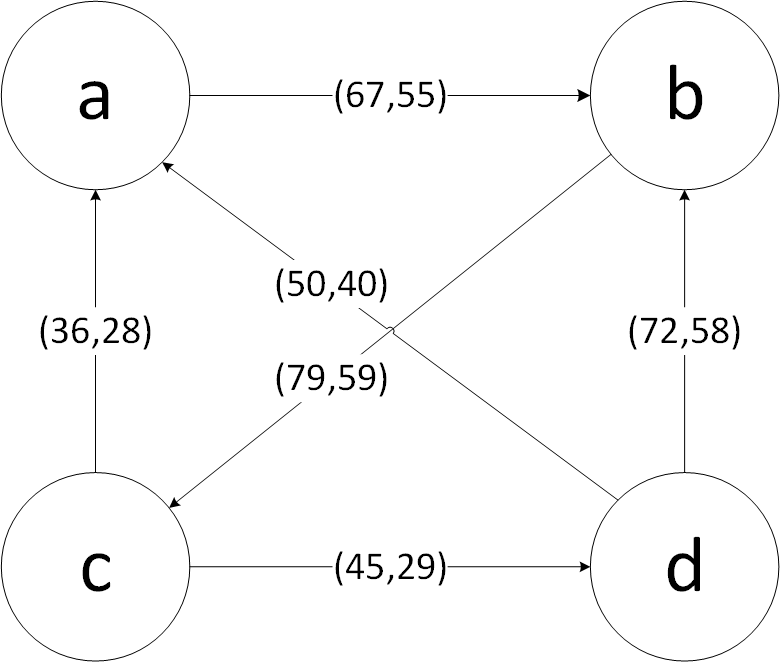
\includegraphics[scale=0.5]{Bilder/Beispiel3_Graph.png}
\caption{Graph über die Menge $N$(Beispiel 3)}
\label{fig:graph3}
\end{figure}

Es gibt vier Möglichkeiten einen Gewinner mit der \schulze zu finden. Wenn alle Wähler die Kandidaten in eine strikte Ordnung gebracht haben, dann geben diese Methoden immer das selbe Ergebnis. Dieses Beispiel ist so aufgebaut, dass jede Methode einen anderen Kandidaten als Sieger ausgibt. Daher ist es wichtig vor der Wahl zu definieren, welche Wahlmethode genutzt wird.

\subsubsection{margin}
\label{sec:margin}
Beim Ansatz $margin$ gewinnt der Kandidat, der seinen Sieg mit einem größeren Abstand erreicht. 
Untersucht wir Beispielhaft das Duell $a$ gegen $b$. Der Stärkste Weg von $a$ nach $b$, ist die direkt Verbindung, Kandidat $a$ erhält 67 Stimmen und Kandidat $b$ nur 55 Stimmen und damit gewinnt Kandidat $a$ mit 12 Stimmen Vorsprung. 
Aber auch Kandidat $b$ kann Kandidat $a$ schlagen, der Stärkste Weg für dieses Duell ist von $b$ über $c$ und $d$ nach $a$. Die schwächste Verbindung in diesem Weg ist die Verbindung $d$ nach $a$, da dort mit nur 10 Stimmen Vorsprung der Kandidat $d$, Kandidat $a$ schlägt.
Um den Gewinner festzustellen wird der Abstand für den Sieg von $a$ (12 Stimmen)mit dem Sieg von $b$ (10 Stimmen) verglichen und der Gewinner dieses Duells ist $a$, mit zwei Stimmen Vorsprung.

Auch hier wurde in Tabelle \ref{beispiel3margin_p} die Menge $P$ aufgestellt. Die Werte in der Tabelle zeigen nun den Abstand, mit dem der Kandidat den Gegner geschlagen hat.

% !TEX root = ../Projektdokumentation.tex
\begin{longtable}[c]{|l|l|l|l|l|}
\hline
            & P{[}*,a{]} & P{[}*,b{]} & P{[}*,c{]} & P{[}*,d{]} \\ \hline
\endfirsthead
%
\endhead
%
P{[}a, *{]} & ---        & 12         & 12         & 12         \\ \hline
P{[}b, *{]} & 10         & ---        & 20         & 16         \\ \hline
P{[}c, *{]} & 10         & 14         & ---        & 16         \\ \hline
P{[}d, *{]} & 10         & 14         & 14         & ---        \\ \hline
\caption{Die Menge $P$ nach margin Regel(Beispiel 3)}
\label{beispiel3margin_p}\\
\end{longtable}

\newpage
Anschließend wird mit den Werten der Menge $P$ die neu Zweikampfsituation erstellt und man erhält die Relation $\mathcal{O}_{margin} = \{ ab, ac,ad,bc,bd,cd \}$

Daraus ergibt sich die Ergebnismenge $\mathcal{S}_{margin} \in \{ a\}$ und er Sieger unter Berücksichtigung des Abstandes ist Kandidat $a$.

\subsubsection{ratio}
\label{sec:ratio}
Eine weitere Methode die eingesetzt wird, um einen Sieger zu erhalten ist ein Verhältnis ( eng: ratio) zu ermitteln. Hierzu werden die Stimmen für den Sieger durch die Stimmen gegen den Sieger geteilt und damit das Verhältnis ausgerechnet, mit dem der Sieger gewonnen hat.

Beispielhaft wird wieder das Duelle von Kandidat $a$ gegen Kandidat $b$ betrachtet. Im Duell $a$ gegen $b$ ist wie im Vergleich über den Abstand (Abschnitt \ref{sec:margin}) der direkte Weg der stärkste Weg. Der Stärkste Weg von Kandidat $b$ zu Kandidat $a$ ist im Vergleich über das Verhältnis aber ein anderer. Er führt von $b$ über $c$ nach $a$ . Die kritische Verbindung ist in diesem Fall die Verbindung von $c$ nach $a$, da hier ein Verhältnis von $36/26 \approx 1,286$, das kleinste Verhältnis auf diesem Weg darstellt. Wird der Weg von Kandidat $b$ nach $a$ aus Abschnitt \ref{sec:margin} untersucht, ist dort die Kritische Verbindung $d$ nach $a$, was ein Verhältnis von $ 50/40 = 1,25$ darstellt und damit eine schlechteres Verhältnis als der Weg $b$ über $c$ nach $a$ hat.

Die Berechnung der besten Verhältnisse wird wieder für alle Duelle gemacht und  Tabelle \ref{beispiel3ratio_p} zeigt die Menge $P$ unter Betrachtung des Verhältnisse.

% !TEX root = ../Projektdokumentation.tex
\begin{longtable}[c]{|l|l|l|l|l|}
\hline
            & P{[}*,a{]} & P{[}*,b{]} & P{[}*,c{]} & P{[}*,d{]} \\ \hline
\endfirsthead
%
\endhead
%
P{[}a, *{]} & ---        & 1,218      & 1,218      & 1,218      \\ \hline
P{[}b, *{]} & 1,286      & ---        & 1,339      & 1,339      \\ \hline
P{[}c, *{]} & 1,286      & 1,241      & ---        & 1,552      \\ \hline
P{[}d, *{]} & 1,25       & 1,241      & 1,241      & ---        \\ \hline
\caption{Die Menge $P$ nach ratio Regel(Beispiel 3)}
\label{beispiel3ratio_p}\\
\end{longtable}

Anschließend wird mit den Werten der Menge $P$ die neu Zweikampfsituation erstellt und man erhält die Relation $\mathcal{O}_{ratio} = \{ ba,bc,bd,ca,cd,da \}$

Daraus ergibt sich die Ergebnismenge $\mathcal{S}_{ratio} \in \{ b\}$ und er Sieger unter Berücksichtigung des Verhältnis ist Kandidat $b$.

\newpage
\subsubsection{winning votes}
\label{sec:winningVotes}
Es kann der Sieger aber auch als die Person gelten, die am meisten Siege hat (eng: winning votes). Dies ist auch das verfahren, welches in den Beispiel 1 (Abschnitt: \ref{sec:beispiel1}) und Beispiel 2 (Abschnitt: \ref{sec:beispiel2}) eingesetzt wurde. Hier wird untersucht, welcher der beiden Kandidaten gewinnt. Exemplarisch tritt wieder Kandidat $a$ gegen Kandidat $b$ an. Kandidat $a$ schlägt Kandidat $b$ mit der Direkten Verbindung mit 67 Stimmen, Kandidat $b$ kann Kandidat $a$ über den Weg $b$ über $c$ und $d$ nach $a$ schlagen. Jedoch ist hier die schwächste Verbindung, die Verbindung $c$ nach $d$ mit nur 45 Stimmen. Diese Werte (Kandidat $a$: 67 Stimmen, Kandidat $b$: 45 Stimmen) werden verglichen und Kandidat $a$ gewinnt. 

Diese Untersuchung wird für alle Duelle gemacht und es ergibt sich die in Tabelle \ref{beispiel3win_p} dargestellte Menge $P$.

% !TEX root = ../Projektdokumentation.tex
\begin{longtable}[c]{|l|l|l|l|l|}
\hline
            & P{[}*,a{]} & P{[}*,b{]} & P{[}*,c{]} & P{[}*,d{]} \\ \hline
\endfirsthead
%
\endhead
%
P{[}a, *{]} & ---        & 67         & 76         & 45         \\ \hline
P{[}b, *{]} & 45         & ---        & 79         & 45         \\ \hline
P{[}c, *{]} & 45         & 45         & ---        & 45         \\ \hline
P{[}d, *{]} & 50         & 72         & 72         & ---        \\ \hline
\caption{Die Menge $P$ nach winning votes Regel(Beispiel 3)}
\label{beispiel3win_p}\\
\end{longtable}


Anschließend wird mit den Werten der Menge $P$ die neu Zweikampfsituation erstellt und man erhält die Relation $\mathcal{O}_{win} = \{ ab,ac,bc,da,db,dc \}$

Daraus ergibt sich die Ergebnismenge $\mathcal{S}_{win} \in \{d\}$ und er Sieger unter Berücksichtigung des Verhältnis ist Kandidat $d$.


\subsubsection{losing votes}
\label{sec:lose}
Ein anderer Ansatz der angewendet werden kann, ist den Kandidaten zum Sieger zu küren, der am wenigsten Gegenstimmen hat (eng. losing votes). Die kritische Verbindung ist dabei die Verbindung, bei der es die meisten Gegenstimmen gibt. Der stärkste Weg ist dann der Weg, bei dem die kritische Verbindung die wenigsten Gegenstimmen hat.

Für dieses Verfahren wird beispielhaft das Duell von Kandidat $a$ und Kandidat $c$ untersucht. Kandidat $a$ kann Kandidat $c$ schlagen über den Weg $a$ über $b$ nach $c$. Dort ist die kritische Verbindung zwischen Kandidat $b$ und $c$, da es an dieser Stelle 59 Gegenstimmen gibt. 
Kandidat $c$ kann Kandidat $a$ über den direkten Weg schlagen und hat dabei nur 28 Gegenstimmen. Die zweite Möglichkeit wäre der Weg von $c$ über $d$ nach $a$, dort wäre die kritische Verbindung von Kandidat $d$ nach $a$ mit 40 Gegenstimmen. Daher wird die Direktverbindung genutzt mit nur 28 Gegenstimmen.
Beide Wege werden nun verglichen und Kandidat $c$ gewinnt gegen Kandidat $a$, da $c$ nur 28 Gegenstimmen hat und Kandidat $a$ 59 Gegenstimmen.

Alle Duelle werde so untersucht, die Ergebnisse, die die Menge $P$ bilden, sind in Tabelle \ref{beispiel3losing_p} eingetragen.

% !TEX root = ../Projektdokumentation.tex
\begin{longtable}[c]{|l|l|l|l|l|}
\hline
            & P{[}*,a{]} & P{[}*,b{]} & P{[}*,c{]} & P{[}*,d{]} \\ \hline
\endfirsthead
%
\endhead
%
P{[}a, *{]} & ---        & 55         & 59         & 59         \\ \hline
P{[}b, *{]} & 59         & ---        & 59         & 59         \\ \hline
P{[}c, *{]} & 28         & 55         & ---        & 29         \\ \hline
P{[}d, *{]} & 40         & 55         & 59         & ---        \\ \hline
\caption{Die Menge $P$ nach losing votes Regel(Beispiel 3)}
\label{beispiel3losing_p}\\
\end{longtable}


Anschließend wird mit den Werten der Menge $P$ die neu Zweikampfsituation erstellt und man erhält die Relation $\mathcal{O}_{los} = \{ ab,ca,cb,cd,da,db \}$

Daraus ergibt sich die Ergebnismenge $\mathcal{S}_{los} \in \{c\}$ und er Sieger unter Berücksichtigung des Verhältnis ist Kandidat $d$.

\subsection{Ergebnis} 
\label{sec:ergebnis3}
Dieses Beispiel zeigt, dass es schwer sein kann zu bestimmen, wann ein Kandidat einen anderen schlägt. Jede Methode ist logisch, korrekt und nachvollziehbar. Dies ist aber nur dann der Fall, wenn man den Wählern erlaubt Kandidaten auch gleich zu bewerten, wenn dies nicht erlaubt ist, ergeben alle vier Methode nach Schulze das selbe Ergebnis, sprich den selben Sieger. Daher muss beachtet werden, dass wenn man Kandidaten gleich bewerten kann, vorher festgelegt werden muss nach welcher Methode man die Stimmen bewertet, da es sonst unter Umständen zu verschiedenen Siegern kommen kann. Dieses Beispiel wurde extra so von Herrn Schulze in seiner Ausarbeitung \glqq A New Monotonic, Clone-Independent,
Reversal Symmetric, and Condorcet-Consistent
Single-Winner Election Method\grqq{} \citep{Schulze2017} konstruiert, dass bei jeder der Methoden unter Abschnitt \ref{sec:loesungen3} immer ein anderer Sieger als Ergebnis geliefert wird, in der Realität kann es auch vorkommen, dass mehrere der vorgestellten Methoden die selben Sieger liefern auch wenn Kandidaten gleich bewertet wurden.
\newpage
% !TEX root = ../Projektdokumentation.tex
\section{Bewertung der Methode}
\label{sec:Bewertung1}

% !TEX root = ../Projektdokumentation.tex
\subsection{Kriterien der Sozialwahltheorie}
\label{sec:kriterienSozial}
Um zu belegen, dass eine Methode gerecht ist, muss eine Methode möglichst viele Kriterien der Sozialwahltheorie erfüllen. Einen kleinen Ausschnitt von Kriterien, die auch in Tabelle \ref{schulzeKramer} aufgeführt sind werden hier erläutert. Eine vollständige Übersicht kann in \glqq The Schulze Method
of Voting\grqq{}\footnote{\Vgl \citet{Schulze2018} Kapitel 11} gefunden werden. Dort wird in Kapitel 4 auch bewiesen, dass die \schulze die Kriterien erfüllt.


\subsubsection{Monotonie Kriterium} 
\label{sec:monotoniekriterium}
Der Gewinner einer Wahl kann nicht durch ein besseres Ranking verlieren und ein Verlierer durch ein schlechteres gewinnen.\footnote{\Vgl \citet{Woodall1996}} Dieses Kriterium ist trivial, aber zeigt, dass die zugrundeliegende Wahlmethode nicht der erwarteten Logik einer Wahl widerspricht.

Das bedeutet, dass wenn die schwächste Verbindung des Siegers stärker werde, kann er dadurch nicht verlieren, dasselbe gilt auch für Verlierer, wenn deren schwächste Verbindungen schwächer werden, dann können sie damit nicht gewinnen.

\subsubsection{\condorcet Kriterium} 
\label{sec:condorectKriterium}
Nach der Wahl wird ein Zweikampf zweier Kandidaten simuliert und dabei untersucht, wie oft der Kandidat $a$ dem Kandidat $b$ vorgezogen wurde. Die Bedeutung von \glqq vorgezogen\grqq{} wir in Abschnitt \ref{sec:beispiel3} für die \schulze erläutert, ist im Allgemeinen aber abhängig von der gewählten Wahlmethode. \condorcetSieger ist der Kandidat, der alle anderen Kandidaten schlägt. Einen solchen Sieger muss es nicht geben. Ein Wahlverfahren erfüllt das Condorcet-Kriterium, wenn der gewählte Sieger auch der \condorcetSieger ist, sofern es einen \condorcetSieger gibt.\footnote{\Vgl \citet{Johnson2005}}

Das Verhalten konnte in Beispiel 1 (Abschnitt \ref{sec:beispiel1}) beobachtet werden, dort wurde auch der Condorcet-Sieger der Sieger der \schulze .

\subsubsection{Lösbarkeitskriterium} 
\label{sec:loesbarkeitsKriterium}
Es gibt Situationen, in denen eine Wahlmethode keinen eindeutigen Sieger hervorbringen kann, da die Stimmsituation für zwei oder mehrere Kandidaten gleich sind. Auch die \schulze kann nicht immer direkt einen eindeutigen Sieger bestimmen. Jedoch kann man mathematisch zeigen, dass eine Methode im Allgemeinen eine eindeutige Lösung liefert.\footnote{\Vgl \citet{Schulze2017}}
\begin{enumerate}
\item Wenn die Anzahl der Stimmen Richtung unendlich tendiert, geht die Wahrscheinlichkeit keinen eindeutigen Sieger zu erhalten gegen Null.
\item Wenn es mehr als einen Sieger gibt, reicht eine einzelne Stimme, um einen eindeutigen Sieger zu erhalten.
\end{enumerate}

Für die Schulz Methode bedeutet zwei Sieger immer, dass zwei Kandidaten nicht geschlagen wurden, beispielsweise die Kandidaten $a$ und $b$. Wenn eine weitere Stimme hinzukommt, die zwischen den beiden Siegern $a$ und $b$ unterscheidet, z.B. Kandidat $a$ wird dem Kandidaten $b$ vorgezogen, so ändert sich die schwächsten Verbindungen zu Gunsten des Kandidaten $a$, sodass nun ein eindeutiger Sieger gefunden werden kann, da $b$ nun von $a$ geschlagen wird.


\subsubsection{Pareto Kriterium} 
\label{sec:paretoKriterium}
Dieses Kriterium gibt an, dass
\begin{enumerate}
\item wenn jeder Wähler Kandidat $a$, Kandidat $b$ vorzieht, muss Kandidat $a$ immer Kandidat $b$ bevorzugt werden
\item wenn kein Wähler Kandidat $a$, Kandidat $b$ vorzieht, muss Kandidat $a$ nicht besser sein als $b$.\footnote{\Vgl \citet{Schulze2017}}

Dieses Prinzip wird wichtig, wenn Kandidaten gleich oder nicht bewertet werden dürfen. Dort darf keine Methode einen der beiden Kandidaten auswählen und ihm eine bestimmte Platzierung geben oder in eine Reihenfolge einordnen. Diese Kandidaten müssen, wenn sie nicht unterschieden werden können, immer auf derselben Ebene eingeordnet werden. 

Dies wird oftmals gebrochen, wenn die Auswertung eine Reihenfolge ausgeben muss und dann einfach der Kandidat der im Alphabet als erstes kommt zuerst anzeigt, oder der der in der Liste als erstes auftaucht. Das muss aber von der Wahlmethode auf jeden Fall unterbunden werden, so wie die \schulze es auch macht. 
\end{enumerate}




% !TEX root = ../Projektdokumentation.tex
\subsection{Vergleich mit anderen Methoden}
\label{sec:alternativeAlgorithmen}

Das Forschungsgebiet der Sozialwahltheorie ist seit dem 19. Jahrhundert ein wichtiges Gebiet, um gerechte Wahlen zu garantieren. Daher gibt es auch eine große Anzahl von anderen Methoden, die einen Sieger hervorbringen. Eine Methode die laut Barry Wright \citep{Wright2009} mit hoher Wahrscheinlichkeit das selbe Ergebnis liefert, wie die \schulze ist die Simpson-Kramer Methode.

Diese Methode erklärt die Person zum Sieger, deren größte Niederlage kleiner war als alle Niederlagen der anderen Kandidaten \citep{Nurmi2017}.  

Wie in Tabelle \ref{schulzeKramer} zu sehen ist, erfüllt diese Methode aufgrund seiner Simplizität nur einen kleinen Teil der Kriterien. Diese Methode kennt man auch unter dem Namen Minmax-Methode.




% !TEX root = Projektdokumentation.tex

\begin{longtable}[c]{|l|l|l|}
\hline
Kriterien &Schulze                       & Simpson-Kramer     \\ \hline
\endfirsthead
%
\endhead
%
resolvability                 & Ja             & Ja   \\ \hline
Pareto                        & Ja             & Ja   \\ \hline
reversal symmetry             & Ja             & Nein \\ \hline
monotonicity                  & Ja             & Ja   \\ \hline
independence of clones        & Ja             & Nein \\ \hline
Smith                         & Ja             & Nein \\ \hline
Smith-IIA                     & Ja             & Nein \\ \hline
Condorcet                     & Ja             & Ja   \\ \hline
Condorcet loser               & Ja             & Nein \\ \hline
majority for solid coalitions & Ja             & Nein \\ \hline
majority                      & Ja             & Ja   \\ \hline
majority loser                & Ja             & Nein \\ \hline
participation                 & Nein           & Nein \\ \hline
MinMax set                    & Ja             & Nein \\ \hline
prudence                      & Ja             & Ja   \\ \hline
polynomial runtime            & Ja             & Ja   \\ \hline
\caption{Vergleich der \schulze mit der Simpson-Kramer Methode.}
\label{schulzeKramer}\\
\end{longtable}

Aus der Tabelle geht hervor, dass es auch die \schulze nicht schafft alle Kriterien zu erfüllen. Jedoch erfüllt die \schulze vielen Anforderungen, die andere Methoden nicht erfüllen. Daher kann man sagen, dass die \schulze eine gute \condorcet Methode ist, um einen Sieger zu ermitteln. Die ausführliche Beschreibung der Kriterien kann in seiner Ausarbeitung aus dem Jahr 2018\footnote{\Vgl \citet{Schulze2018}} nachgelesen werden, aus der auch diese Tabelle abgeleitet wurde.
\newpage

\subsection{Eindeutigkeit}
\label{sec:eindeutigkeit}
Die \schulze wurde als eine Methode vorgestellt, die einen Sieger ermittelt. Jedoch ist das nicht ganz richtig. Es kann auch vorkommen, dass zwei Sieger gefunden werden. Wenn man eine Situation wie diese

\begin{description}
\centering
\item[3 mal] $a \succ_{v} b \succ_{v} c \succ_{v}d$
\item[2 mal] $c \succ_{v} b \succ_{v} d \succ_{v}a$
\item[2 mal] $d \succ_{v} a \succ_{v} b \succ_{v}c$
\item[2 mal] $d \succ_{v} b \succ_{v} c \succ_{v}a$
\end{description} 
untersucht, erhält man nicht einen Sieger sondern zwei, $\mathcal{S}=\{b,d\}$. Die \schulze bietet keine Möglichkeit einen eindeutigen Sieger in dieser Situation zu ermitteln. In diesen Fällen wird geraten eine Stichwahl zwischen den Kandidaten durchzuführen. Da die \schulze aber das Lösbarkeitskriterium  aus Abschnitt \ref{sec:loesbarkeitsKriterium} erfüllt, würde ein weiterer Wahlzettel, der zwischen den Kandidaten eindeutig unterschiedet zu einem eindeutigen Ergebnis führen.

% !TEX root = ../Projektdokumentation.tex
\newpage
\section{Bewertung des Algorithmus}
\label{sec:Bewertung2}

% !TEX root = ../Projektdokumentation.tex
\section{Implementierung}
\label{sec:implementierung}

Der Autor hat eine mögliche Implementierung der \schulze in Java entwickelt. Die untenstehende Implementierung arbeitet nach der ''winning votes'' Methode, die in Beispiel 3 in Abschnitt \ref{sec:winningVotes} beschrieben wird. Wie in Beispiel 3 (Abschnitt: \ref{sec:beispiel3}) zu erkennen ist, gibt es auch für die anderen Möglichkeiten einen Sieger zu bestimmen.

Eine Vollständige Implementierung kann man auf Gitub finden.\footnote{\url{https://github.com/SteffenHo/SchulzeImplementation}} Dort sind auch Beispielaufrufe hinterlegt. 

\lstinputlisting[language=JAva,numbers=none]{Listings/Schulze.java}

\subsection{Laufzeit}
\label{sec:Laufzeit}
Die Laufzeitkomplexität der \schulze ist mit $O(C^3)$ nicht besonders gut, wobei C die Anzahl der Kandidaten ist. Diese Komplexität sieht man auch in der Implementierung in Abschnitt \ref{sec:implementierung}, dort wird über mit einer dreifach verschachtelten Schleife über ein Array iteriert. Jedoch ist die Laufzeit zu relativieren, da diese Methode zum auswerten einer Wahl nur einmal laufen muss, um ein Ergebnis zu liefern.

Auch wird die Zahl der Kandidaten meist nicht ins unendliche steigen, da es in normalen Wahlen eine endlich oft recht begrenzte Anzahl von Kandidaten gibt. Trotzdem muss man die Komplexität beachten, wenn man die \schulze in Systeme einbaut, die nicht einer klassische Abstimmung, wie es sie z.B. in Politik gibt, entsprechen und C beliebig groß werden kann.



% !TEX root = ../Projektdokumentation.tex
\newpage
\section{Fazit}
\label{sec:Fazit}

\subsection{Eingangsbeispiel}
Ganz zu Beginn (Abschnitt \ref{sec:problemstellungBeispiel}) wurde eine Wahlsituation von 30 Wählern und 3 Kandidaten beschrieben, die auf den ersten Blick kein Sieger geliefert hat. Die Wahl kann mit der \schulze ausgewertet werden und liefert auch Kandidat $a$ als Sieger. Der Unterschied, die naive Idee, $a$ zu nehmen weil der Kandidat auch viele Zweitstimmen hatte, fühlt sich gerecht an. Die \schulze kann mathematisch beweisen, dass sie nach bestimmten Kriterien gerecht ist.

\subsection{Einsatz} 
\label{sec:einsatz}
Erstmals wurde die \schulze 2003 im Debian, eine Linux Distribution, eingesetzt. Dort waren es ca. 1000 Wahlberechtigte, die ihre Wahlen mit dieser Methode auswerten.\footnote{\Vgl \citet{Debian2018}} Sie nutzen die \schulze z.B. um bestimmte Features auszuwählen. Beispielsweise wurde im Jahr 2014 mit der \schulze über das Init-System für Debian abgestimmt.\footnote{\Vgl \citet{Leemhu2014}}



2008, 2009 und 2011 wurde die \schulze von Wikimedia, den Dachverband von Wikipedia, genutzt, um zu entscheiden wer die Führung der Organisation übernehmen soll. Es waren im Jahr 2011 43.000 Wahlberechtigte. \footnote{\Vgl \citet{Schulze2017}}

Auch in der Politik hat diese Methode ihre Heimat gefunden. 2009 hat die Piratenpartei von Schweden diese Wahlmethode eingeführt, 2010 die Piratenpartei Deutschland, 2011 die Australische Piratenpartei, 2013 die Piratenpartei Island, 2015 die niederländische Piratenpartei.\footnote{\Vgl \citet{Lohmann2013}}

Die \schulze hat sich über die Jahre zu der am weitesten verbreiteten \condorcet Methode entwickelt. Über 60 Organisationen mit über 800.000 Wahlberechtigten nutzen diese Methode.\footnote{\Vgl \citet{Schulze2018}} Des weiteren arbeiten auch einige online Tools damit, wie z.B. GoogleVotes, bei denen man nicht genau beziffern kann, wie viele Wahlberechtigte diese Tools generieren.\footnote{\Vgl \citet{Hardt2015}}








\input{Inhalt/Erklärung}


% Literatur ------------------------------------------------------------------
\clearpage
\renewcommand{\refname}{Literaturverzeichnis}
\bibliography{Literatur}
\bibliographystyle{Allgemein/natdin} % DIN-Stil des Literaturverzeichnisses


% Anhang ---------------------------------------------------------------------
\clearpage
\appendix
\pagenumbering{roman}
% !TEX root = Projektdokumentation.tex
\section{Anhang}
\subsection{Erster Anhang}
\label{app:ersteranhang}




\end{document}
